\documentclass[12pt,letterpaper]{article}

%Packages
% \usepackage{textcomp}
% \usepackage{latexsym}
% \usepackage{url}
% \usepackage{amssymb}
% \usepackage{amsmath}
% \usepackage{mathtools}
% \usepackage{bm}
% \usepackage{array}
% \usepackage[version=3]{mhchem}
% \usepackage{ifthen}
% \usepackage{amsthm}
% \usepackage{amstext}
% \usepackage{enumerate}
% \usepackage{dcolumn}

\usepackage{epsfig}
\usepackage{graphicx}
\usepackage{caption}
\usepackage{hyperref}
\usepackage{lineno}
\usepackage{pdflscape}
\usepackage{mathtools}
\usepackage[osf]{mathpazo}
\usepackage{fullpage}
\usepackage{float}
\usepackage{xr} %linking to supplementaries
\externaldocument{supplementaries}

\pagenumbering{arabic}


%---------------------------------------------
%
%       START
%
%---------------------------------------------

\begin{document}
%Running head
\begin{flushright}
Version dated: \today
\end{flushright}

\bigskip
\bigskip
\begin{center}

\noindent{\Large \bf Innovation and elaboration on the avian tree of life}
\bigskip

\noindent {\normalsize \sc Thomas Guillerme$^{1,*}$, Natalie Cooper$^{2}$, Andrew P. Beckerman$^{1}$, and Gavin H. Thomas$^{1,3}$}\\
\noindent {\small \it 
$^1$School of Biosciences, University of Sheffield, Sheffield, S10 2TN, United Kingdom.\\
$^2$Natural History Museum, Cromwell Road, London, SW7 5BD, United Kingdom.\\
$^3$Bird Group, Department of Life Sciences, the Natural History Museum at Tring, Tring, United Kingdom.\\}


\end{center}
\bigskip
\noindent{*\bf Corresponding author.} \textit{guillert@tcd.ie}\\ 
\vspace{1in}

%Line numbering
\modulolinenumbers[1]
\linenumbers

%---------------------------------------------
%
%       ABSTRACT
%
%---------------------------------------------


% New narrative:
% 1 - Novelty arises through elaboration and innovation
% 2 - Theory suggests that it is easier to evolve along the major axis of variation (formely LOTR in this manuscript)
% 3 - However this has never been tested in big datatests. We do that.
% 4 - We measure elaboration and innovation in all birds
% 5 - We find that there is more elaboration than innovation
% 6 - But that asks another (more interesting) question: why do we have diversity if everything elaborates?
% 7 - We then measure novelty by clades rather than by species
% 8 - We find that clades innovate.
% 9 - So basically species elaborate (in line with the micro evol theory of evolving along the line for major axis of variation) and clades innovate (in line with the observations at a macro and mega level of evolutionary jumps leading to big diversity at high levels). 



\noindent (Keywords: macroevolution, elaboration, innovation, variance-covariance matrices, line of least resistance, GLMM)\\

\section{Abstract}

Patterns of biological diversity across the tree of life are the result of millions of years of evolutionary history and are shaped by natural selection.
A long-standing proposal is that most morphological diversity at a macroevolutionary scale (among species) arises along a microevolutionary ``line of least resistance''.
At macro- and mega-evolutionary scales, however, we frequently observe major shifts in phenotypes among lineages \cite{venditti2011multiple, pagel2022general}.
The presence of distinct morphological forms suggests instead that species or clades may evolve away from the line of least resistance.
At a macroevolutionary level, evolution along a common major axis has been termed elaboration whereas evolution away from the major axis is termed innovation \cite{endler2005animal, renaud2006conserved}.
The extent to which elaboration and innovation contribute to phenotypic diversity among species and clades is critical to our understanding of the origins and maintenance of biodiversity across scales from the micro- to macro and mega-evolutionary.
Here we apply new multi-trait methods to modelling the traits nested covariance structure to evaluate the magnitude and distribution of elaboration and innovation in the evolution of bird beaks among species and clades.
Our analyses show that elaboration dominates species-level phenotypic divergence which is consistent with micro-evolutionary theory.
However, we also find that innovation is relatively common at the clade level suggesting multiple routes to specific phenotypic innovation throughout avian evolutionary hiostory.
These results show that although phenotypic elaboration and innovation occur throughout evolutionary scales, elaboration seems to dominate at the micro-evolutionary scales and innovation is more prevalent at the macro-evolutionary scale.
This interaction suggest that both innovation and elaboration are ubiquitous routes for phenotypic change at any scale and are a common evolutionary route that explain both the amazing avian diversity and phenotypic conservatism.
%TG: bleuargh...

% TODO in abstract, add the "paradox" bit: However, if most organisms evolve incrementally along stable lines of least resistance then how can we explain the staggering diversity of species morphologies across the tree of life?


\section{Main}

% paragraph 1:  introducing the major axis of variation + novelty and innovation
Evolutionary theory predicts that over short, microevolutionary, timescales phenotypic evolution will tend to follow evolutionary lines of genetic least resistance \cite{schluter1996adaptive}.
Over longer timescales, the evolutionary line of least resistance is analogous to the major axis of phenotypic variation \cite{marroig2005size,fasanelli2022allometry}.
Numerous studies show that phenotypic divergence is biased along the genetic line of least resistance, and therefore reflects the major axis of phenotypic variation, over 1-2 million year timescales.
%TG: cite some of these numerous studies.
Recent evidence suggests that this stability can even extend over macroevolutionary timescales spanning tens of millions of years \cite{mcglothlin2018adaptive}.
However, while the line of least genetic resistance explicitly reflects genetic constraints, the macroevolutionary major axis of phenotypic variation is an emergent property of genomic and developmental constraints interacting with selection on a moving adaptive landscape \cite{jones2004evolution}.
The widespread evidence of major shifts in phenotypes across the tree of life \cite{pagel2022general,cooney2017mega,venditti2011multiple,khabbazian2016fast,smaers2021evolution} suggests a tension in the direction of phenotypic evolution across scales where macroevolutionary divergence away from the major axis of phenotypic variation results in megaevolutionary divergence leading to distinct phenotypes and/or directions of evolution.
Resolving this tension requires an understanding of the balance between deep-time reorientation of phenotypic major axes of evolution among clades and the directions of evolution of species within clades.

% paragraph 2:  introducing the Endler view.
Endler et al. \cite{endler2005animal}, writing in the specific context of signal evolution, describe two routes to phenotypic novelty that we suggest can help to illuminate this challenge.
Specifically, Endler et al. refer to evolution of new phenotypes along the same major axis of phenotypic variation as \textit{elaboration}.
This is akin to phenotypic divergence among species following lines of least resistance, and, by definition, would be expected to be a major driver of phenotypic evolution.
In contrast, they refer to evolution away from the major axis of phenotypic variation as \textit{innovation}.
More specifically they describe new phenotypes falling "off the line in random directions" as \textit{random innovation} and new phenotypes falling "off the line in only one direction (or a few)" as \textit{specific innovation}.
For example, studies of allometry in which the allometric slope varies among clades \cite{marroig2005size,Rombaut2022}
%TG: potential add Marcy et al 2020 as a ref here too (hidden self-cite)?
are consistent with specific innovation.
Relative to elaboration, both random and specific innovation may be more likely to generate phenotypic novelty, but this need not be synonymous with being a primary driver of phenotypic diversity at broad scales.
These core concepts provide a powerful theoretical framework with which to study macro- to mega-evolutionary divergence and in particular to determine the relative importance of:
i) idiosyncratic species-level change (random innovation) against clade-level reorientation of the directions of phenotypic variation (specific innovation),
and ii) evolution along versus away from major axes of phenotypic variation.
The contributions of these multivariate evolutionary pathways are poorly-known despite their importance for understanding the origins of diversity from macro- to mega-evolutionary scales. 
Here we assess the stability of trait correlations across the global radiation of birds and estimate and compare major axes of beak shape evolution across lineages and scales to address the contributions of elaboration and innovation to the generation of avian phenotypic diversity.
 
% paragraph 3: how we measure this (glmm) on the birds data + nestedness
\subsection{Modelling nested trait covariances}
Addressing the relative contributions of elaboration and innovation to the origins of biodiversity in deep-time requires
1) large, multivariate datasets to allow exploration of trait covariances at different scales,
2) reliable and efficient computational methods to estimate the major axes of phenotypic variation,
and 3) a set of mathematical tools that can estimate degrees of elaboration and both random and specific innovation at any scale.
To meet the first challenge we use an eight-dimensional beak shape morphospace based on a geometric morphometric dataset of 8748 species of birds (described in \cite{hughes2022global}).
To meet the second two challenges we propose a novel analytical pipeline for measuring elaboration and random innovation at the species level and both elaboration and specific innovation at the clade level (Fig.S\ref{Fig:cheat_sheet} and S\ref{Fig:mcmcmcglmm}).
To provide a baseline from which to calculate elaboration and innovation (i.e. the major axis of phenotypic variation) we use phylogenetic generalised mixed effect models (pGLMM) with beak shape as an eight-dimensional response variable (see Methods; \cite{MCMCglmm}).
Such models allow us to measure variance-covariance matrices partitioned into phylogenetic and non-phylogenetic components. 
From these models we can calculate major axes of phenotypic variation as the leading eigenvector of the variance-covariance matrix in trait space.
We regard the major axis of phenotypic variation as a deep-time analogue of the microevolutionary \textbf{G} matrix and posit that it represents the line of least evolutionary resistance capturing the effects of historical contingency on multivariate evolution.
The major axis of phenotypic variation can be defined at any phylogenetic scale (i.e. for all species in the phylogeny, or for all species within any monophyletic clade).
To assess the roles of elaboration and innovation across scales we fit our pGLMM as nested models in which we define variance-covariance matrices (and therefore major axes of phenotypic variation) for
i) the entire phylogeny of all species included in the data (hereafter the global phylogenetic level),
ii) all species within each of nine clades mapping approximately to super-orders (the super-order level),
and iii) all species within each of 27 clades mapping to taxonomic orders (the order level).
These nested partitions of multivariate trait space provide the basis for all subsequent analyses.

\subsection{Elaboration dominates species-level divergence}
% paragraph 4: results for elaboration and innovation for species
We tested the expectation, derived from adaptive radiation theory, that species divergence is biased along lines of least resistance by calculating species specific measures of random innovation and elaboration.
To do this we calculated the multilinear algebraic projection of each species phenotype onto the three major axis of phenotypic variation (global phylogeny, specific super-order, and specific order).
Phylogenetic distributions of random innovation and elaboration broadly hold whether comparisons are made at the order, super-order, or global phylogenetic level (Fig. \ref{Fig:phylogeny})%{#fig_correlations}),%TODO: maybe add to supp?
 and in further nested analysis of the order Passeriformes (Fig. S\ref{fig_ellipses_passeriformes} and S\ref{fig_phylogeny_passeriformes}).
However, the extent of both elaboration and random innovation tends to reduce as we move from global phylogeny to within order comparison.
Broadly, and not surprisingly, this trend reflects the fact that species are more similar to the major axis of phenotypic variation of their close relatives than to the major axis of phenotypic variation of all birds.
The global phylogenetic major axis of phenotypic variation aligns closely with the major axis in the trait space and primarily describes variation between short, deep, and wide beaks at one extreme and long, shallow, and narrow beaks at the other.
Our results point to the possibility that within clades the major axes of phenotypic variation follow different directions. 

Overall we found that, as expected, elaboration is the dominant mode of divergence at the species level \ref{Fig:phylogeny}.
We find no consistent evidence that innovation is either positively correlated with, or trades-off with, elaboration. %(Fig. S{#fig_correlations}). %TODO: maybe add to supp? 
However, we observe various combinations of elaboration and random innovation across birds.
Examples of high innovation and/or elaboration are often clustered within clades.
For example, compared to global phylogenetic major axis of phenotypic variation, the Trochilidae (hummingbirds) in the order Apodiformes, have long narrow beaks and display high levels of elaboration and low innovation.
In contrast, the Bucerotiformes (hornbills), with large and deep beaks display high levels of innovation and low elaboration.
Other clades such as the Apodidae (swifts) in the order Apodiformes and the distantly related but convergent Hirundidae (swallows and martins) have exceptionally wide (relative to length) beaks and display high levels of both elaboration and specific innovation.
The dominance of elaboration when measured at the species level is consistent with idea of evolution along lines of least evolutionary resistance.
However, the frequent clustering of species that elaborate, innovate, or both, again highlights the likelihood that major axes of phenotypic variation are not stable among clades.
This leads us to ask: if most organisms evolve incrementally along major axis of phenotypic variation then how can we explain the staggering diversity of species morphologies across the tree of life? 

\begin{figure}[!htbp]
\centering
    \includegraphics[width=0.9\textwidth]{Figures/InnovElabTree_main_text.pdf}
\caption{.}
\label{Fig:phylogeny}
\end{figure}


\bigskip

\noindent \textbf{Figure \ref{Fig:phylogeny}:} The avian phylogeny (n=8748 species) coloured by species beak shape innovation and elaboration level.
Blue and yellow colors highlight species with relatively low novelty whereas orange to red colours indicate high novelty.
The novelty is represented as innovation (upper circle) and elaboration (lower circle) concentrically represented in a nested fashion with the most external pairs of circles (innovation and elaboration bands) representing novelty for each species at the order levels then at the super-order level and finally at the entire phylogeny level.
We can observe an increase of novelty at deeper phylogenetic with novelty consistently composed of more elaboration than innovation.
%TODO: add density plots of the innovations and elaboration at different levels.
The branches are coloured by the species distance from the centroid of the shapespace and the estimation of their ancestors' position in that space.
A companion plot showing further nested structure within the Passeriformes is shown in Fig. S\ref{fig_phylogeny_passeriformes}.

\subsection{Multiple routes to specific innovation throughout avian evolutionary history}

To investigate the tension implied by our observations of species-level elaboration and previously reported deep time jumps in phenotype, we measured the elaboration and specific innovation of different clades.
To do this we translated the major axes of phenotypic variation of each clade's (i.e. super-orders and orders) phylogenetic variance-covariance matrices onto the global phylogenetic major axis of phenotypic variation so that they shared the same origin in the shapespace.
We then used multilinear algebra to project a focal clade's major axis of phenotypic variation onto the global phylogenetic major axis of phenotypic variation (Fig.S\ref{Fig:cheat_sheet}).
We interpret the measured projection (distance onto the phylogenetic major axis of phenotypic variation) as the clade's elaboration score and the measured rejection (distance from the major axis of phenotypic variation) as the clade's specific innovation score.
These scores were measured for each of 4000 posterior pairs of clade vs. phylogenetic variance-covariance matrix (Fig.\ref{Fig:ellipses} boxplots).
We found that for most clades the phenotypic major axis of phenotypic variation is not aligned with the global phylogenetic major axis of phenotypic variation (Fig. \ref{Fig:ellipses}). 
Despite the limitations representing eight-dimensional space in 2D, our plots of the average elliptical representation of the phenotypic variance-covariance matrix for the global phylogenetic major axis of phenotypic variation and each super order (Fig. \ref{Fig:ellipses}a) and order (Fig. \ref{Fig:ellipses}b) highlight the variation in the orientation of phenotypic evolution among clades (Fig. \ref{Fig:orthogonality}).
Remarkably, more than half of the assessed clades (4/8 super-orders and 15/27 orders) displayed higher median innovation than median elaboration scores implying that, contrary to micro-evolutionary theory \cite{schluter1996adaptive,marroig2005size}, specific innovation is a more common generator of morphological diversity than elaboration in deep time.
However, there is substantial variation in elaboration and innovation across clades including relatively low elaboration and innovation (e.g. Cuculiformes; Fig. \ref{Fig:ellipses}), low elaboration and high innovation (e.g. Galliformes; Fig. \ref{Fig:ellipses}), high elaboration and low innovation (e.g. Coraciiformes; Fig. \ref{Fig:ellipses}) or both relatively high elaboration and innovation (e.g. Podicipediformes; Fig. \ref{Fig:ellipses}).
These patterns hold across scales including within super-orders and at finer scales within the order Passeriformes (Fig. S\ref{fig_ellipses_passeriformes}).
Our observations of heterogeneity in the orientation of the major axis of phenotypic variation among clades is further supported by consistent evidence for orthogonality of clades relative to the major phylogenetic axis of phenotypic variation (Fig. \ref{Fig:ellipses} - Fig. \ref{Fig:orthogonality}).
The median angle of the major axis of phenotypic variation for subclades approaches orthogonality, differing from the phylogenetic major axis of phenotypic variation by $68.14^\circ$ ($95$\% CI: $22.83^\circ$-$89.09^\circ$ - Fig. \ref{Fig:orthogonality}).
Comparisons of orientation among subclades (i.e. orders within super-orders) show similar differences (median = $47.14^\circ$; $95$\% CI: $13.64^\circ$-$87.62^\circ$ - Fig. \ref{Fig:orthogonality}), suggesting that reorientations in trait space are largely unconstrained at the megaevolutionary level and are no more likely to occur along any one axis than another.
This differs from previous inference on a subset of our data that implied generally consistent and low dimensionality within clades \cite{cooney2017mega}.
This suggests that there is no deep time analogue of the evolutionary line of least evolutionary resistance and that across scales there is a remarkable flexibility in the routes to innovation, consistent with the idea that morphological divergence may be less constrained in deep-time than is often assumed \cite{venditti2011multiple}.




\begin{figure}[!htbp]
\centering
   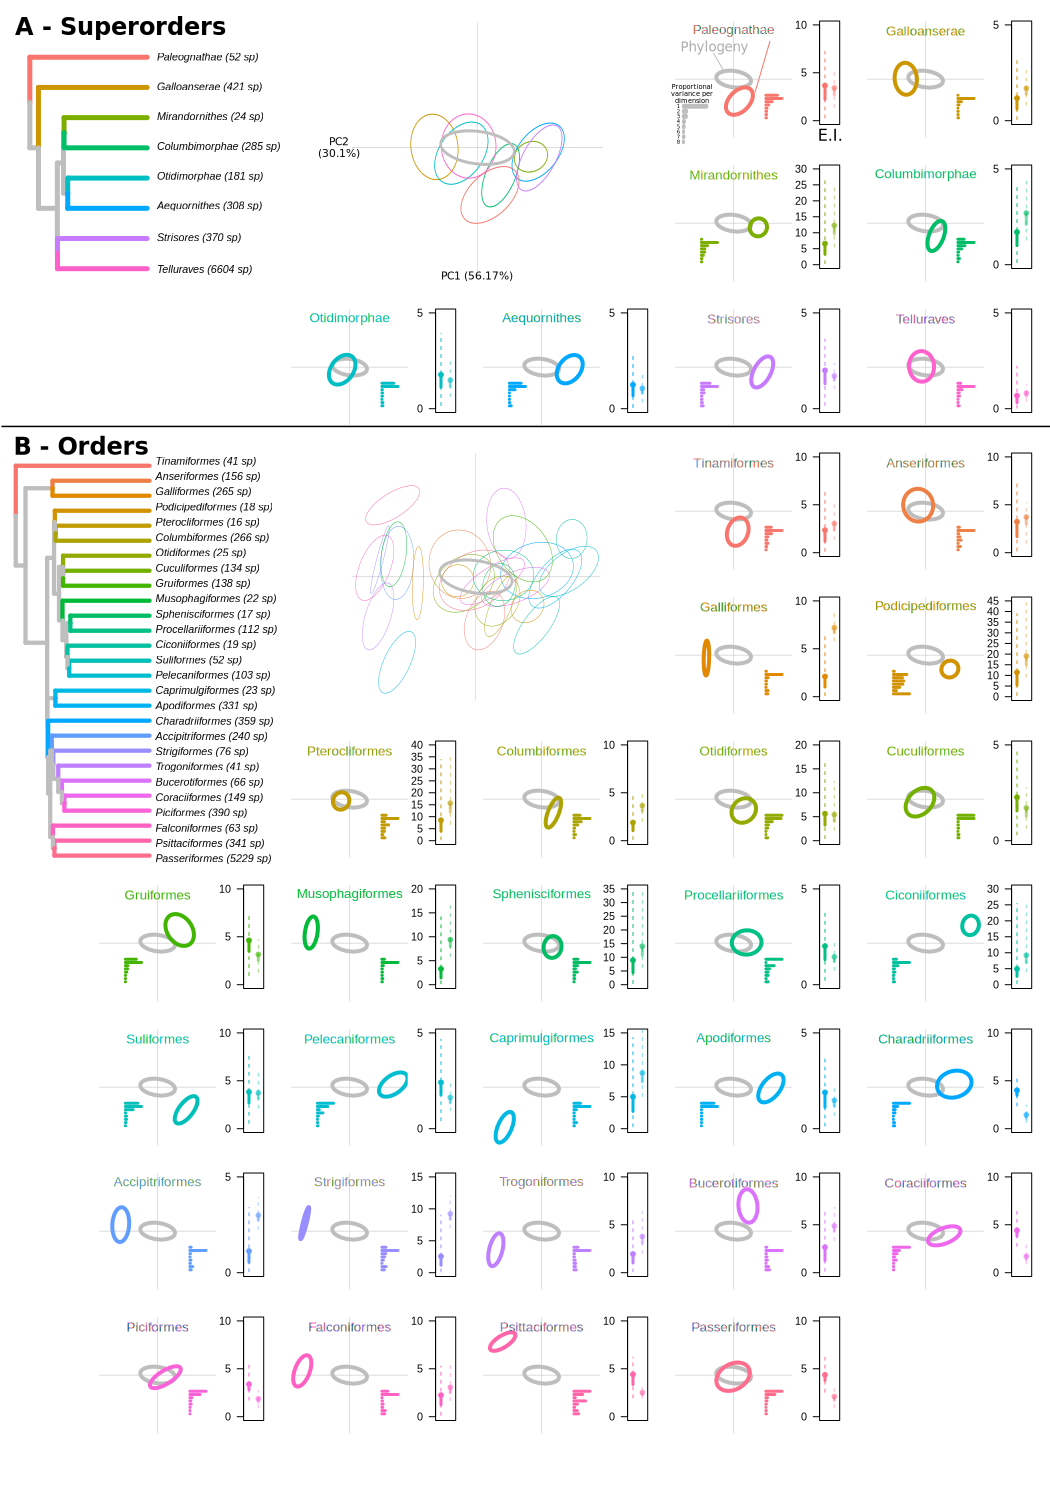
\includegraphics[width=1\textwidth]{Figures/ellipses.pdf}
\caption{.}
\label{Fig:ellipses}
\end{figure}
\bigskip

\noindent \textbf{Figure \ref{Fig:ellipses}:}
Panel A) shows ellipses representing the scaled average posterior variance-covariance response from the pGLMM models for each super-order (coloured ellipses) compared to the all-birds phylogenetic component of the models (grey ellipses)
We scaled the ellipses so the length of the major axis of phenotypic variation of the clade ellipses is the same length as that of the global ellipse (in eight dimensions).
The first inset ellipse plot shows the positions of all super-order ellipses relative to the all-bird phylogenetic ellipse.
Subsequent inset plots show the results for each super-order. Inset barplots show the proportion of variance associated with each of the eight PC axes in shape morphospace.
The inset boxplots correspond to the elaboration (E) and innovation (I) scores for all 4000 posterior samples.
The dots represent the median elaboration and innovation values while the thick and dashed lines represent the 50\% and 95\% confidence intervals respectively.
Note that these scores were calculated on the unscaled ellipses resulting in different scales of elaboration and innovation scores for each plot. %TG: TODO: add figure with unscalled ellipses in the supplementaries
Panel B) shows the results for each order.
A companion plot showing further nested structure within the Passeriformes is shown in Fig. S\ref{fig_ellipses_passeriformes}.

\bigskip

\bigskip





\begin{figure}[!htbp]
\centering
   \includegraphics[width=0.9\textwidth]{Figures/orthogonality_results.pdf}
\caption{.}
\label{Fig:orthogonality}
\end{figure}

\bigskip

\noindent \textbf{Figure \ref{Fig:orthogonality}:}
Orthogonality of each clade's major axis of phenotypic variation compared to their parent or parent parent's clade.
Orthogonality is represented on the horizontal axis scales from 0 (modulo of $0^\circ$) to 1 (modulo of $90^\circ$) with the background grey and dashed grey lines represent respectively an orthogonality of 0.5 (modulo of $45^\circ$) and 0.75 (modulo of $67.5^\circ$).
Dots represent the clades median orthogonality and the lines their 95\% CI.
No super-order's major axis of phenotypic variation is parallel to the global phylogeny (red lines and circles) and 12/25 orders are at least half orthogonal to their super-order (green lines and circles).
These results are even clearer when comparing them to the global phylogeny (green dashed lines and open circles) where only 3/25 are not at least half orthogonal.
Furthermore we also indicate here the number of species (n) and the standard deviation of their major axes of phenotypic variation orientation over the 4000 variance-covariance posteriors (sd; expressed in degrees).
For each clade we also measured the posterior propbabilityof each clade's orientation being different from their parent's clade or the global phylogeny relative to their sample size and sd.
The stars represent the posterior probability of the clade's orientation being different from the comparison clade. (*** = pp $> 0.99$; ** = pp $>0.95$; * = pp $> 0.9$; . = pp $> 0.8$).
Only two out of six super-orders; 6/25 orders relative to their super-order and 9/25 orders relative to the phylogeny have a pp $> 0.99$.
This is the result of a variation of sample size (n) and standard variation (sd) between clades. 
A companion plot showing further nested structure within the Passeriformes is shown in Fig. S\ref{fig_orthogonality_passeriformes}.
%TG: TODO: very easy low hanging fruit (maybe?), but not for this paper is to plot orthogonality through time.

\bigskip


The inferred evolutionary innovation can arise in any direction in trait space.
Although the global phylogenetic major axis of phenotypic variation aligns closely with the first dimension (70.96\% of the global phylogenetic major axis of phenotypic variation is aligned on PC1; Fig. \ref{Fig:ellipses}) of the raw shapespace, no super-order, and only seven of the 27 orders (Procellariiformes, Pelecaniformes, Charadriiformes, Coraciiformes, Psittaciformes and Passeriformes), follow this trend Fig. \ref{Fig:ellipses}-bar plots).
This also holds for sub-orders and families within the Passeriformes where only half of the sub-orders (Meliphagoidea, Corvides and Passerida) and seven out of the 23 families (Eurylaimides, Meliphagoidea, Petroicidea, Fringilidae, Aegithaloidea, Pyconotiae, Nectariniidae) align with the Passeriformes PC1 (Fig. S\ref{fig_ellipses_passeriformes}).
In addition to the variable alignment of clade major axes of phenotypic variation, we further found that within clades, phenotypic variation is either highly constrained (varying almost entirely along a single axis) or higher-dimensional than expected from the global phylogenetic variance-covariance matrix.
For example, Accipitriformes (hawks and allies) have major axes of phenotypic variation that mainly align with the second dimension of the shapespace suggesting distinct directions of evolution for the clade relative to the global phylogeny but uniformity in their beak shape components within the clade.
In contrast, the Podicipediformes (grebes) are highly variable across all dimensions suggesting that all components of the shapespace are necessary to describe their beaks.
These observations illustrate multiple routes to innovation and imply that reorientations of trait space can arise in any direction, in any lineage, and at any time throughout avian history.


\subsection{Species elaborate, clades innovate OR Ubiquitous elaboration, clade innovation}

% Paragraph 7: putting these results together

The disconnect between observations of reorientation of trait space at the clade level and a dominance of elaboration at the species level could be viewed as a paradox.
We formalise this paradox by testing whether elaboration is more common at higher taxonomic levels than at the species level.
We compared the area under the curve of the scaled density of elaboration and innovation at both the species level and the clade level.
We then measured the difference between both areas and found that there was a significant difference in innovation between species and clades but no clear difference in elaboration (Fig. \ref{Fig:relative_EI}).
This difference confirms our observation that while specific innovation is common and perhaps even dominant at the clade level, elaboration (rather than random innovation) dominates at the species level. So, although species evolve preferentially along a shared major axis of phenotypic variance, this major axis changes frequently among clades.
However, we suggest that rather than a paradox the reorientation of trait space can instead arise as a result of small innovations that arise in a common direction among closely related species.
This idea is similar in concept to models of multiple adaptive peak models where species evolve in a heterogenous adaptive landscape and share similar responses to selection pressures within adaptive zones.
%GT: Tip-toeing into OU territory and needs citations but I think this is a fair suggestion. %TG: fair point!
This implies that gradual directional evolution \cite{pagel2022general}, rather than exceptional megaevolutionary jumps \cite{cooney2017mega,venditti2011multiple}, may be sufficient to explain diversity in avian beak morphology.

\begin{figure}[!htbp]
\centering
   \includegraphics[width=0.9\textwidth]{Figures/relative_EI.pdf}
\caption{.}
\label{Fig:relative_EI}
\end{figure}

\bigskip

\noindent \textbf{Figure \ref{Fig:relative_EI}:} Comparisons of relative elaboration and innovation among clades (illustrated in figure  \ref{Fig:ellipses}) and among species (figure \ref{Fig:phylogeny}).
A - In blue, the elaboration for each species in each 4000 posterior samples compared to the elaboration for each 35 clades.
The scores for each clade is scaled by the maximum score within each clade (corresponding to the scaled ellipses in figure  \ref{Fig:ellipses}) and the score for the species is scaled by the maximum species elaboration score.
This allows us to compare both types (species vs. clades) despite their different sample sizes.
The Bhattacharryya Coefficient represents the overlap of the area under the curve for species and clades (a BC of 0 represents no overlap).
B - same as A but for the innovation score.
We can see a clear difference in the amount of innovation across the posterior samples between species or clades.


% Paragraph 8: conculsion
\subsection{Conclusions}

Our results show that although at the species level most bird beaks are elaborating along a mega-evolutionary major axis of phenotypic variation, at the macro-evolutionary level innovation way from the major axis of phenotypic variation is much more common. 
This nested structure of elaboration at a higher taxonomic level and innovation at a lower taxonomic level could thus explain the diversity of bird beaks we observe today.
However, individual species-level variation in the past could also have led to a shift in a clade's line of least evolutionary resistance through different evolutionary routes on a dynamic adaptive landscape. 
Taken together, our results suggest that the signature of evolutionary orientations in deep-time, coupled with elaboration at the species-level, is consistent with recent suggestions that apparently abrupt phenotypic shifts observed in univariate analyses can be explained by gradual Darwinian processes \cite{pagel2022general}.
Indeed, the global phylogenetic major axis of phenotypic variation is an emergent property of reorientation of trait space among clades that requires no special evolutionary process: megaevolutionary patterns appear to be an inevitable outcome of microevolution on a shifting adaptive landscape. 



\section{Methods}


\textbf{Beak shape data.}
We used the dataset from \cite{cooney2017mega,chira2020signature,hughes2022global} which consists of four landmarks and three curves of 25 semi-landmarks each, taken from 3D scans of  the beaks of 8748 bird species.
The landmark data were aligned with Procrustes superimposition using the R package \texttt{Morpho} \cite{Rcore,Morpho} and we removed the size component and controlled for symmetry (see \cite{cooney2017mega,chira2020signature,hughes2022global} for detailed descriptions of data collection and processing).
We ordinated the superimposed landmarks using a principal components analysis (PCA) and selected the eight first dimensions of the resulting PCA.
These eight dimensions contained at least 95\% of variance in each super-order, and 98.7\% of the variance in the whole dataset.
We used a threshold of $>95$\% of variance explained for each super-order because although the overall distribution of the variance on each PC axis in the whole trait-space is decreasing (i.e.
$\sigma$ PC1 $<$ $\sigma$ PC2 $<$ $\sigma$ PC3), this is not always true for each super-order.
For example, in the Mirandornithes, PC2, then PC4, and then PC1 contained the most variance (Fig. \ref{Fig:ellipses} and S\ref{Fig:axes_variance}).
This protocol for selecting the number of PC axes ensures that the resulting trait-space contains enough variance for each super-order (see Fig. S\ref{Fig:axes_variance} and Table \ref{tab_variance_per_axis}).
This procedure resulted in an $8748 \times 8$ matrix that contains at least 95\% of the variance in all observed living bird beaks (hereafter, the shapespace).

\textbf{Phylogenetic data.}
We used a random subsample of 1000 trees from the avian tree distribution of \cite{jetz2012global} for the analyses and the one randomly selected tree for the figures (Fig. \ref{Fig:phylogeny}).
We pruned these trees to contain only the 8748 species present in our beak shapespace.




\textbf{Phylogenetic GLMM analysis.}
We ran a phylogenetic Bayesian generalised linear mixed effects model (pGLMM) using the \texttt{MCMCglmm} R package \cite{MCMCglmm} with the shapespace data as a multidimensional response variable, the error in the dataset as residuals, and each clade's phylogeny as a nested random term, i.e., a model of:

\begin{equation}
\text{shapespace} \mathtt{\sim} \text{residuals(shapespace)} + \text{random(phylogeny)}
\end{equation}

This model allows us to estimate a phenetic variance-covariance matrix for each clade and the phylogeny as a whole, and one for the residuals in the shapespace itself \cite{robinson2013quantifying}.
These variance-covariance matrices were then used in a base projection-rejection analysis to measure the elaboration and innovation scores (see below).
We ran two separate nested models.
One model using one random term for the global phylogeny and 35 nested random terms for each super-order and order containing more than 15 species in our dataset (Fig. \ref{Fig:ellipses}).
And one model on a subset of the dataset containing only the 5229 passeriformes species with 30 nested random terms.
This resulted in two multidimensional GLMM.
One with a $8748 \times 8$ response variables, one global residual term and 36 random terms.
And one with a $5229 \times 8$ response variable, one global residual term and 30 random terms.
 
To account for phylogenetic uncertainty we needed to run the model using different tree topologies from the tree distribution in \cite{jetz2012global}.
Because of the very large size of our model and dataset, however, running the full model on multiple trees was computationally unfeasible (it would require 2 CPU years and 4TB of RAM for each - the global phylogeny and the passeriformes ones).
Instead, we developed and implemented a ''mini chains'' MCMCglmm method using the R package \texttt{mcmcmglmmm} \cite{mcmcmcglmmm}.

\textbf{mcmcmcglmm.}
This method consists in running relatively short monte-carlo markov chains (MCMC) across a large number of different phylogenetic trees and concatenating the resulting short posteriors into one larger one that contains the phylogenetic uncertainty information.
This was effectively done in four steps (see Fig. S\ref{Fig:mcmcmcglmm})
1) running three independent MCMCglmm chains (hereafter the parametrisation chains) for 50k generations with the traits data and the model described above on the consensus tree from the tree distribution, along with flat priors with a belief parameter of 2\% (effectively not a very low weight on the priors);
2) extracting the following parameters from the parameterisation chains:
a) the conservative burnin average time (across the three chains) defined as the highest number of iterations required to first reach the median posterior likelihood value multiplied by 1.1; and
b) the mini-chains priors defined as the median posterior model values from the parameterisation chains with a belief parameter of 5\%.
We then ran 400 mini chains in parallel with the estimated burnin time and priors in order to just run 10 samples past the burnin.
This effectively resulted in getting 10 exploitable posterior samples per tree.
We used 400 trees because that was the number of models required to reach an effective sample size (ESS) of at least 200 for all the estimated parameters (see Fig. S\ref{Fig:model_ess_all_birds} and S\ref{Fig:model_ess_passeriformes}).
Using this approach, we reduced the computational time to around 45 CPU hours and 9GB of RAM per mini-chain (a 400 fold improvement).
The whole procedure is reproducible in the \href{https://raw.rawgit.net/TGuillerme/mcmcmcglmmm/main/inst/MCMCglmm_mini_chains.html}{\texttt{mcmcmcglmmm} vignette} \cite{mcmcmcglmmm}.

\textbf{Projection/rejection analyses.}
We used the distributions of the 4000 posterior variance-covariance matrices to run the projection/rejection analyses to measure the bird beaks' elaboration and innovation scores.
In fact we can use multilinear algebra to interpret elaboration and innovation \textit{sensu} \cite{endler2005animal} by using the major axis of the variance-covariance matrices as the ''line of least resistance'', or, specifically here, the line of elaboration for each random terms (corresponding to the elaboration axes for each clade) and project either species or other major axis of phenotypic variation onto that clade.
In brief we can interpret where a species or a clade falls on the major axis of phenotypic variation of reference as its elaboration score and how far a species is from that major axis of phenotypic variation as its innovation score.
We calculated the elaboration and innovation scores using two main approaches:
1) by clades (i.e. to measure the elaboration/innovation between clades) where we calculated the projections of the major axes of each clade onto the global phylogenetic major axes of phenotypic variation (Fig. \ref{Fig:ellipses});
and 2) by species (i.e. to measure the elaboration/innovation within clades) where we calculated the projections of each species onto a) the global phylogenetic major axes of phenotypic variation and b) the whole tree's major axes of phenotypic variation of their respective clade (Fig. \ref{Fig:phylogeny}).
To make the results easier to interpret, we centered and scaled them onto the centre of the major axis of phenotypic variation of interest and made the elaboration values absolute.
This way, we can interpret an elaboration or innovation score within the 0-1 range to be not exceptional (i.e within the 95\% confidence interval of the variance-covariance matrix).
The entire mathematical procedure is described in details in the supplementary materials (section \ref{supp_projection}).
The whole procedure applied to our dataset is reproducible in \href{https://raw.rawgit.net/TGuillerme/dispRity/master/inst/vignettes/Projection_analysis.html}{this \texttt{dispRity} vignette} % TODO: update link to release when releasing
and implemented in the \texttt{dispRity} package \cite{dispRity}.

\textbf{Groups' orthogonality.}
We measured the orthogonality of each random term in our models (clades) compared to their parent clade and their parent parent's.
For example, the Columbimorphae random terms' variance-covariance matrices against the phylogeny ones, the Columbiformes ones against the Columbimorphae ones (parent) and the whole phylogeny ones (parent parents).
To do so we measured the angles between the major axes of phenotypic variation of the focal clade and their parent clade for each posterior variance-covariance matrix as well as within each clade by randomly comparing major axes of phenotypic variation within a clade.
We converted each angle measurement into an orthogonality metric where 0 corresponds to flat angles ($0^\circ$ or  $180^\circ$) and 1 to right angles ($90^\circ$ or $270^\circ$).
We then measured the posterior probability of the angles within a clade being different than the angles between clades.
These results are available in Fig. \ref{Fig:orthogonality}.

\textbf{Reproducibility and repeatability.}
The raw and processed data used in this analysis is available from \href{https://figshare.com/articles/dataset/Innovation_and_elaboration_on_the_avian_tree_of_life/20480355}{figshare} \cite{fighsaredata}.
The code used to reproduce the figures and tables is available from \href{https://github.com/TGuillerme/elaboration_exploration_bird_beaks}{github} \cite{githubrepo}.

\textbf{Funding.}
This work was funded by UKRI-NERC Grant NE/T000139/1 and a Royal Society University Research Fellowship (URF R 180006 to GHT).


\bibliographystyle{naturemag}
\bibliography{references}


\end{document}